\chapter{Introduction and motivation}\label{cha:introduction_and_motivation}

\section{Outline of the problem}\label{sec:outline_of_the_problem}

Better camera calibration improves the performance of various downstream tasks
by providing a more accurate mapping between 3D world coordinates and 2D image
plane coordinates. This improved mapping enables precise alignment, positioning,
and scaling of objects within the scene. By determining the camera's intrinsic
and extrinsic parameters, algorithms can correct for lens distortion, estimate
depth information, and accurately overlay virtual content. Consequently, tasks
such as 3D reconstruction, augmented reality, and object detection can achieve
better results in terms of precision, spatial consistency, and overall visual
quality.

Although manufacturers can estimate camera calibration parameters a priori,
fully automatic calibration is often preferred, especially when camera metadata
is unavailable. Currently, wide-angle lenses, particularly in mobile phones and
GoPro-type cameras, dominate consumer photography. These cameras pose additional
challenges due to their requirement for highly non-linear models with numerous
parameters. The high distortion of the image plane also makes finding key points
robustly challenging.

Typically, camera calibration is obtained by capturing an image of a known
calibration pattern, which is then used to estimate the camera parameters.
Alternatively, some methods do not use a calibration pattern but instead, infer
geometric constraints directly from the scene. However, this approach is
generally less accurate.

As reported by \textcite{duisterhofTartanCalibIterativeWideAngle2022} on
\citedate{duisterhofTartanCalibIterativeWideAngle2022}, the current state-of-the-art
methods
\citep{olsonAprilTagRobustFlexible2011, schopsWhyHaving102020,
	krogiusFlexibleLayoutsFiducial2019}
fail on images with high distortion.
\cite{duisterhofTartanCalibIterativeWideAngle2022} suggested an iterative
the approach of image undistortion and target reprojection, achieving the superior
robustness to the noise than the state-of-the-art methods because the feature
detection is performed on the undistorted image.

Instead of searching for the features on the undistorted image from scratch, it
is possible to utilize the prior knowledge of the geometry of the calibration
board, effectively predicting the possible positions of previously undetected
features. It can be done by projecting the board onto the image using the
intermediate camera calibration, and then filtering the possible positions in
order to eliminate false positives.

These additional points will further constrain the camera calibration, improving
the accuracy of the calibration parameters.

\begin{figure}
	\begin{tikzpicture}[spy using outlines={circle,yellow,magnification=4,size=3cm, connect spies}]
		\node[anchor=south west,inner sep=0] (image) at (0,0)
		% {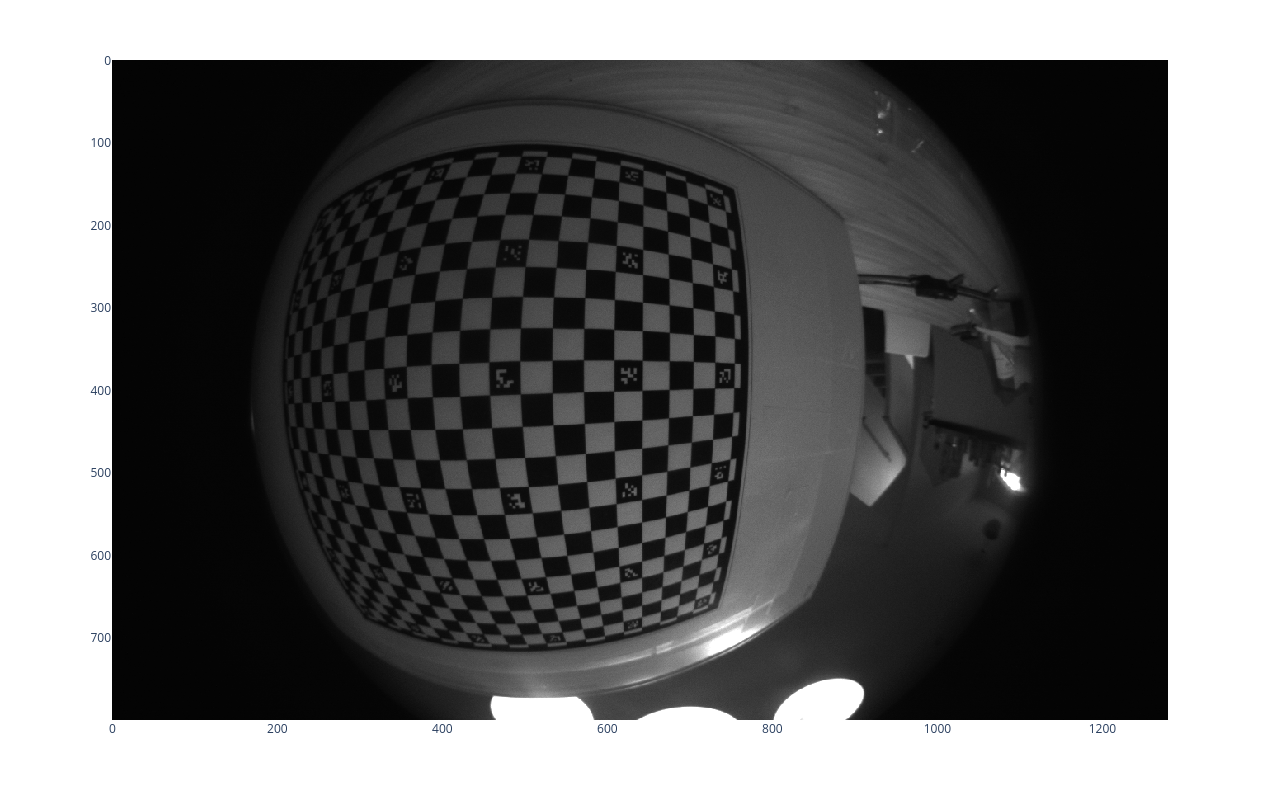
\includegraphics[width=0.6\textwidth]{distorted_image}};
		{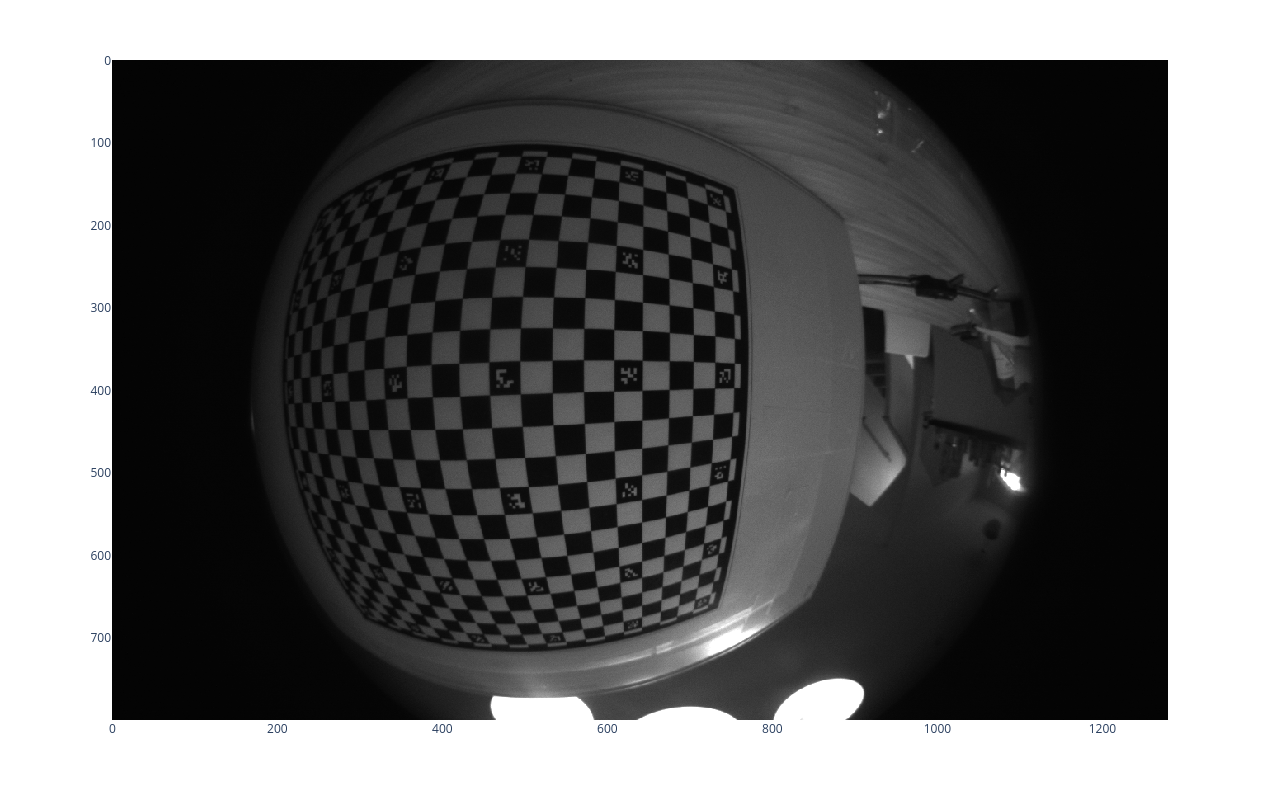
\includegraphics[width=0.8\textwidth]{distorted_image}};
		\begin{scope}[x={(image.south east)},y={(image.north west)}]
			\spy[red] on (3.3,1.7) in node [left] at (10.1,1.7);
			\spy[blue] on (4.6,3.2) in node [right] at (8.1,5.3);
		\end{scope}
	\end{tikzpicture}
	\caption{Example of corners near the center of the image and the edge}
\end{figure}

\section{Research objective}\label{sec:research_objective}

The objective of this research is to add additional constrains to the camera
calibration by finding previously undetected features on the calibration
board. For that, we formulate the set of research questions:
\begin{itemize}
	\item How to find additional features on the calibration board which were not
	      detected by the feature detector?
	\item How to filter out falsely detected features?
  \item Is there a need for finding additional features on the calibration
    board? Are all of the points detected?
\end{itemize}

\section{Thesis structure}\label{sec:thesis_structure}

This paper has the following structure: in \cref{related_work}, we will describe
various subtopics of the camera calibration, and outline the current state-of-the-art solutions.
In \cref{cha:background}, we will describe the key concepts of camera
calibration. Also, there we provide additional details on the underlying math,
for example, the derivation of the division model inversion. In
\cref{cha:approach}, we will describe the steps of the proposed method in
detail, including feature detection, initial camera calibration, camera
parameters estimation via minimization of the reprojection error, and the
process of searching and filtering the previously undetected features. In
\cref{Experiments}, we will describe the metrics we used, provide details about
the datasets, show the results of each of the algorithm's steps, and evaluate it
on multiple metrics. Finally, in \cref{cha:conclusions}, we will summarize the
results and outline future work.


